%%%%%%%%%%%%%%%%%%%%%%%%%%%%%%%%%%%%%%%%%
% Jacobs Portrait Poster
% LaTeX Template
% Version 1.0 (31/08/2015)
% (Based on Version 1.0 (29/03/13) of the landscape template
%
% Created by:
% Computational Physics and Biophysics Group, Jacobs University
% https://teamwork.jacobs-university.de:8443/confluence/display/CoPandBiG/LaTeX+Poster
% 
% Further modified by:
% Nathaniel Johnston (nathaniel@njohnston.ca)
%
% Portrait version by:
% John Hammersley
%
% The landscape version of this template was downloaded from:
% http://www.LaTeXTemplates.com
%
% License:
% CC BY-NC-SA 3.0 (http://creativecommons.org/licenses/by-nc-sa/3.0/)
%
%%%%%%%%%%%%%%%%%%%%%%%%%%%%%%%%%%%%%%%%%

%----------------------------------------------------------------------------------------
%	PACKAGES AND OTHER DOCUMENT CONFIGURATIONS
%----------------------------------------------------------------------------------------

\documentclass[final]{beamer}

\usepackage[scale=1.24]{beamerposter} % Use the beamerposter package for laying out the poster
\usepackage[utf8]{inputenc}

\usepackage{relsize}

\usetheme{confposter} % Use the confposter theme supplied with this template

\setbeamercolor{block title}{fg=ngreen,bg=white} % Colors of the block titles
\setbeamercolor{block body}{fg=black,bg=white} % Colors of the body of blocks
\setbeamercolor{block alerted title}{fg=white,bg=dblue!70} % Colors of the highlighted block titles
\setbeamercolor{block alerted body}{fg=black,bg=dblue!10} % Colors of the body of highlighted blocks
% Many more colors are available for use in beamerthemeconfposter.sty

%-----------------------------------------------------------
% Define the column widths and overall poster size
% To set effective sepwid, onecolwid and twocolwid values, first choose how many columns you want and how much separation you want between columns
% In this template, the separation width chosen is 0.024 of the paper width and a 4-column layout
% onecolwid should therefore be (1-(# of columns+1)*sepwid)/# of columns e.g. (1-(4+1)*0.024)/4 = 0.22
% Set twocolwid to be (2*onecolwid)+sepwid = 0.464
% Set threecolwid to be (3*onecolwid)+2*sepwid = 0.708

\newlength{\sepwid}
\newlength{\onecolwid}
\newlength{\twocolwid}
\newlength{\threecolwid}
\setlength{\paperwidth}{36in} % A0 width: 46.8in
\setlength{\paperheight}{48in} % A0 height: 33.1in
\setlength{\sepwid}{0.024\paperwidth} % Separation width (white space) between columns
\setlength{\onecolwid}{0.22\paperwidth} % Width of one column
\setlength{\twocolwid}{0.464\paperwidth} % Width of two columns
\setlength{\threecolwid}{0.708\paperwidth} % Width of three columns
\setlength{\topmargin}{-0.5in} % Reduce the top margin size
%-----------------------------------------------------------

\usepackage{graphicx}  % Required for including images

\usepackage{booktabs} % Top and bottom rules for tables


\usepackage{lmodern} 
\usepackage{amsmath}
\usepackage{amssymb}
\usepackage{graphicx}

\usepackage[T1]{fontenc}

\DeclareFontShape{OMX}{cmex}{m}{n}{
  <-7.5> cmex7
  <7.5-8.5> cmex8
  <8.5-9.5> cmex9
  <9.5-> cmex10
}{}

\SetSymbolFont{largesymbols}{normal}{OMX}{cmex}{m}{n}
\SetSymbolFont{largesymbols}{bold}  {OMX}{cmex}{m}{n}

%----------------------------------------------------------------------------------------
%	TITLE SECTION 
%----------------------------------------------------------------------------------------

\title{Connectionist Temporal Classification: \\Labelling Unsegmented Sequences with \\Recurrent Neural Networks} % Poster title

\author{Thomas Mesnard, Alex Auvolat} % Author(s)

\institute{Probabilisitc Graphical Models Project, MVA Master} % Institution(s)

%----------------------------------------------------------------------------------------

\begin{document}

\addtobeamertemplate{block end}{}{\vspace*{2ex}} % White space under blocks
\addtobeamertemplate{block alerted end}{}{\vspace*{2ex}} % White space under highlighted (alert) blocks

\setlength{\belowcaptionskip}{2ex} % White space under figures
\setlength\belowdisplayshortskip{2ex} % White space under equations

\begin{frame}[t] % The whole poster is enclosed in one beamer frame

\begin{columns}[t] % The whole poster consists of three major columns, the second of which is split into two columns twice - the [t] option aligns each column's content to the top

\begin{column}{\sepwid}\end{column} % Empty spacer column

\begin{column}{\twocolwid} % Begin a column which is two columns wide (column 2)

\begin{columns}[t,totalwidth=\twocolwid] % Split up the two columns wide column

\begin{column}{\onecolwid}\vspace{-.6in} % The first column within column 2 (column 2.1)

%----------------------------------------------------------------------------------------
%	MATERIALS
%----------------------------------------------------------------------------------------


\begin{block}{Abstract}

Many real-world sequence learning tasks require the prediction of sequences of
labels from noisy, unsegmented input data. Recurrent
neural networks (RNNs) are powerful sequence learners that would seem well
suited to such tasks. However, because they require pre-segmented training
data, and post-processing to transform their outputs into label sequences,
they cannot be applied directly. CTC is a method
for training RNNs to label unsegmented sequences directly, thereby solving both
problems.

\end{block}


%----------------------------------------------------------------------------------------

\end{column} % End of column 2.1

\begin{column}{\onecolwid}\vspace{-.6in} % The second column within column 2 (column 2.2)

%----------------------------------------------------------------------------------------
%	METHODS
%----------------------------------------------------------------------------------------

\begin{block}{Main Idea}

RNNs are powerful learners for sequences, but:

\begin{itemize}
\item Standard methods need pre-segmented training data
\item Need for complex post-preprocessing
\end{itemize}

CTC solves this problem:

\begin{itemize}
\item Able to train RNNs using unsegmented training data
\item Learns the segmentation automatically
\item Provides directly usable output
\end{itemize}

This method is now extremely used, even by Google!

\end{block}


%----------------------------------------------------------------------------------------

\end{column} % End of column 2.2

\end{columns} % End of the split of column 2 - any content after this will now take up 2 columns width

%----------------------------------------------------------------------------------------
%	IMPORTANT RESULT
%----------------------------------------------------------------------------------------

\begin{alertblock}{The problem and how CTC solves it}

\begin{figure}
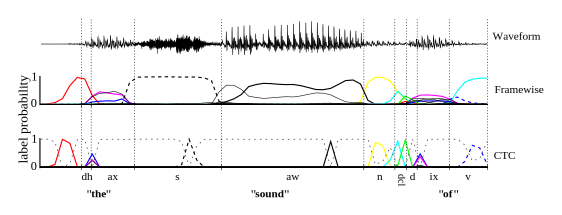
\includegraphics[width=0.9\linewidth]{azerty3.png}
\caption{\small Output of classic framewise phoneme classification and RNN trained with CTC}
\end{figure}

\end{alertblock} 

%----------------------------------------------------------------------------------------


\begin{block}{Model}
\begin{columns}[t,totalwidth=\twocolwid] % Split up the two columns wide column again


\begin{column}{\onecolwid} % The first column within column 2 (column 2.1)

\begin{itemize}
\item Cost function for RNNs
\item RNN outputs probabilities for the different symbols, plus blank symbol
\item Many possible alignments for the correct label (shorter than input)
\item Dynamic programming: sums all the possible alignments
\item Provides gradients for the RNN to learn a good alignment
\end{itemize}

\vspace{1em}
\begin{figure}
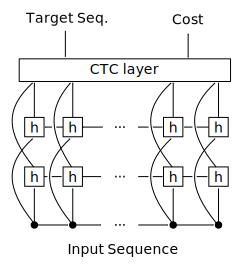
\includegraphics[width=0.8\linewidth]{azerty4.png}
\caption{Simple bidirectional RNN model with CTC cost layer}
\end{figure}

%----------------------------------------------------------------------------------------

\end{column} % End of column 2.1

\begin{column}{\onecolwid} % The second column within column 2 (column 2.2)


CTC is a dynamic programming algorithm that calculates the following sum:
\[
\alpha_t(s) = \sum_{\substack{\pi \in N^T :\\\mathcal{B}(\pi_{1:t}) = l_{1:s}}} 
	\prod_{t'=1}^t y_{\pi_{t'}}^{t'}
\]

Where $\mathcal{B}$ is the transform that removes blanks and duplicates.

\begin{figure}
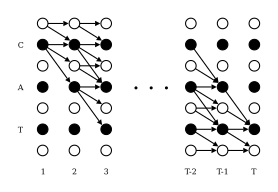
\includegraphics[width=\linewidth]{azerty1.png}
\caption{Computation graph for $\alpha_t(s)$ (corresponds to an unrolled automaton)}
\end{figure}

Tools used for our implementation:
\begin{itemize}
\item Theano (GPU computation library)
\item Blocks (deep learning framework)
\end{itemize}

%----------------------------------------------------------------------------------------

\end{column} % End of column 2.2

\end{columns} % End of the split of column 2

\end{block}

\end{column} % End of the second column



\begin{column}{\sepwid}\end{column} % Empty spacer column



%=================================================================

\begin{column}{\twocolwid} % Begin a column which is two columns wide (column 2)

\begin{block}{Recurrence equations}

\begin{columns}[t,totalwidth=\twocolwid] % Split up the two columns wide column
\begin{column}{\onecolwid} % The first column

We define the following notation:

$y_k^t$: output at time $t$ for symbol $k$

$l$: label, $l'$: label with blanks

Initialization:
\[
\begin{tabular}{rcl}
$\alpha_1(1)$ &=& $y_b^1$\\
$\alpha_1(2)$ &=& $y_{l_1}^1$\\
$\alpha_1(s)$ &=& $0, \forall s > 2$
\end{tabular}
\]

Recurrence relation:
\[
\alpha_t(s) = 
\begin{cases}
	\bar{\alpha}_t(s) y_{l'_s}^t \mbox{ \; if } l'_s = b\mbox{ or }l'_{s-2}=l'_s \\
	(\bar{\alpha}_t(s)+\alpha_{t-1}(s-2)) y_{l'_s}^t \\
		\hspace{3em} \mbox{ otherwise}\\
\end{cases}
\]
\[
\bar{\alpha}_t(s) = \alpha_{t-1}(s) + \alpha_{t-1}(s-1)
\]

Finally, we have:
\[
p(l|x) = \alpha_T(|l'|) + \alpha_T(|l'|-1)
\]

\end{column}
\begin{column}{\sepwid}\end{column} % Empty spacer column
\begin{column}{\onecolwid} % The third column

\begin{figure}
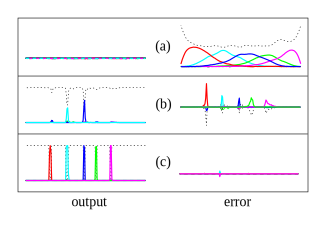
\includegraphics[width=\linewidth]{azerty2.png}
\caption{Evolution of the CTC error signal}
\end{figure}

To avoid numerical underflow, at each step $t$:
\[
C_t = \sum_s \alpha_t(s)
\hspace{1em}
\hat{\alpha}_t(s) = \frac{\alpha_t(s)}{C_t}
\]

Other solution: do calculations in the logarithmic domain. 


\end{column} % End of column 2.2

\end{columns} % End of the split of column 2


\end{block}

\begin{columns}[t,totalwidth=\twocolwid] % Split up the two columns wide column
\begin{column}{\onecolwid} % The first column

\begin{block}{Toy dataset}

We first tried our implementation on a simple task:

{\centering
$1^*2^*3^*4^*5^* \to 1$  \\
$1^*2^*3^*2^*1^* \to 2$  \\
$5^*4^*3^*2^*1^* \to 3$  \\
$5^*4^*3^*4^*5^* \to 4$  \\
}

\begin{itemize}
\item A RNN can easily solve this
\item It needs to read the full sequence before predicting a label
\item CTC provides satisfactory results
\end{itemize}

\begin{table}
\vspace{2ex}
\begin{tabular}{l l l}
\toprule
\textbf{Results} & \textbf{train} & \textbf{valid}\\ 
\midrule
Sequence length & 5 -- 20 & 5 -- 20 \\
Error rate & 0.62 & 0.63 \\
Mean edit distance & 1.0 & 1.1 \\ 
Errors per character & 0.08 & 0.09 \\
\bottomrule
\end{tabular}
\caption{Performances of CTC on our toy dataset}
\end{table}

\begin{figure}
\includegraphics[width=\linewidth]{ctc_cost_best.png}
\caption{Training and validation cost of the CTC model (negative log likelihood)}
\end{figure}
\end{block}

\begin{block}{Conclusion}
CTC is a very powerfull model, and also has a nice mathematical formulation. It is also very used in practice (most successfull applications: speech recognition, handwriting recognition).
\end{block}

%------------------------------------------------


%----------------------------------------------------------------------------------------

\end{column} % End of the first column

\begin{column}{\sepwid}\end{column} % Empty spacer column


\begin{column}{\onecolwid} % The third column

\begin{block}{TIMIT}

We then tried on the classical TIMIT dataset:

\begin{itemize}
\item Raw speech signal dataset
\item Labelled by phonemes or by words
\item 4120 sentences
\item Average audio length: 50000 samples
\item Avg. sentence length: 38 phonemes
\end{itemize}

Model:

\begin{itemize}
\item Convolution layers on raw signal
\item Bidirectional LSTM layers
\item Dropout and noise for regularization
\item CTC cost function
\end{itemize}

This model avoids hand-crafted feature extraction on the speech signal. However it is extremely complicated to train such models. Our model hasn't converged yet.

\end{block}



%\setbeamercolor{block alerted title}{fg=black,bg=norange} % Change the alert block title colors
%\setbeamercolor{block alerted body}{fg=black,bg=white} % Change the alert block body colors

\setbeamercolor{block title}{fg=red,bg=white} % Change the block title color
\begin{block}{Contact Information}

\begin{itemize}
\item Web: \url{http://github.com/thomasmesnard/CTC-LSTM}
\item Email: \url{thomas.mesnard@ens.fr}
			 \url{alex.auvolat@ens.fr}
\end{itemize}

\end{block}

\setbeamercolor{block title}{fg=red,bg=white} % Change the block title color
\begin{block}{References}

\nocite{*} % Insert publications even if they are not cited in the poster
\small{\bibliographystyle{unsrt}
\bibliography{sample}\vspace{0.75in}}


\end{block}

% LOGOS
%\begin{center}
%\begin{tabular}{ccc}
%\includegraphics[width=0.4\linewidth]{logo.png} & \hfill & \includegraphics[width=0.4\linewidth]{logo.png}
%\end{tabular}
%\end{center}

%----------------------------------------------------------------------------------------

\end{column} % End of the third column

\end{columns} % End of all the columns in the poster

\end{column} % End of the third column

\end{columns} % End of all the columns in the poster

\end{frame} % End of the enclosing frame

\end{document}
